\chapter{METHOD OF MEASUREMENTS}\label{cha:measurements}
In this chapter the methods used for testing the mobile devices for different characteristics is described in~\chapterref{cha:character}. Different test where performed to get sensor data to analyze for bias and characteristics. \\
\\
Overview of the tests performed:
\begin{itemize}
  \item[] \textbf{Measurement I - Motion:} Collected accelerometer and gyroscope data by using a JavaScript web-page. The purpose to find out which of \texttt{accelerationIncludingGravity} and \texttt{acceleration} is better in purpose of extract unique device characteristics.
  \item[] \textbf{Measurement II - Motion:} Collected accelerometer and gyroscope data by using a JavaScript web-page. The purpose to find unique device characteristics from the sensors. 
  \item[] \textbf{Measurement II - Camera:} Collect one video from each device and extract pictures frames from the video. Calculate and compare the PRNU of the extracted pictures. (The videos where collected in the same process as test II above).
  \item[] \textbf{Measurement III - Camera:} Collected ten pictures instead of video from the device. 
\end{itemize}

\section{Measurements of sensors on mobile devices}\label{sec:charMeasureSensor}
Measurements of sensors from mobile devices can be gather in different ways. In the work of this thesis two approaches is used, a browser application and an Android application. The camera is an exception where pictures provides the sensor characteristics.
\begin{figure}[H]
	\centering
    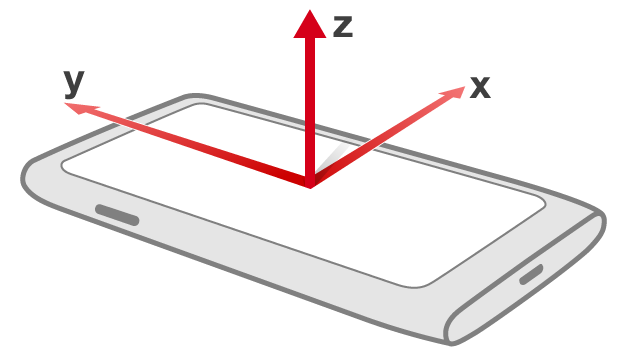
\includegraphics[scale=0.2]{img/device-axes}
    \caption{The coordinate system used for both Android and JavaScript\cite[]{sensor:W3C}}
  \label{fig:device-axes}
\end{figure}

\subsection{Android}\label{subsec:Android}\index{Android}
\textbf{==== OBS: Är detta mer relevant att ha i demo-delen?} \\
Android sensor framework provides raw data with high precision from sensor that are built in the device such as different motions sensors (including accelerometer and gyroscope), environmental sensors and position sensors (e.g. magnetometer). \cite[]{android:sensor}
Android sensor framework classes that is used for gather sensor data is; 
\begin{itemize}
	\item[] \texttt{SensorManager}, a manager used to access the sensor of the device. 
	\item[] \texttt{Sensor}, representing a sensor
	\item[] \texttt{SensorEvent}, an event from a Sensor such data from the sensor, time-stamp or accuracy
	\item[] \texttt{SensorEventListener}, gets a SensorEvent when a sensor or accuracy has changed 
\end{itemize}
In Android you can't just read from the sensor whenever you need, instead the SensorEventListener has a function that is triggered every time the sensor is changed. You can however set how fast the delay from the sensor should be. The function provides the output of the sensor with a time-stamp of when (in nanoseconds) the change occurred. The template code for this function:
\lstinputlisting[caption={Java code for Android sensor},label={code:androidSensor},language=Java]{code/android-sensor.java}
\cite[]{android:sensorEvent} 




\subsubsection{Accelerometer in Android}\label{subsec:accAndroid}
\texttt{TYPE\_ACCELEROMETER} is the hardware measurements that measures the force of acceleration including the force of gravity with the SI unit $m/s^2$. Android also provide \texttt{TYPE\_LINEAR\_ACCELERATION} that is without gravity but that is a combined hardware and software sensor, thus this tests uses  \texttt{TYPE\_ACCELEROMETER} were the measurements only comes from hardware. There have been some bias removal from the sensor such bias from different temperature. \\
To get the acceleration applied to the device ($a_d$) the measurements of the force ($F_s$) applied the sensor is calculated from Newtons second law using the mass ($m$) of the device :
$$a_d=-\sum F_s / m $$ 
These measurements from the \texttt{SensorEvent} is in the x-,y- and z-axes like in~\figureref{fig:device-axes} and collected from event like x=a, y=b and z=c in~\coderef{code:androidSensor}. \cite[]{android:sensorEvent}


\subsubsection{Gyroscope in Android}\label{subsec:gyroAndroid}
The data from the gyroscope sensor is collected from the \texttt{TYPE\_GYROSCOPE} that measures the rotation in rad/s around the x-, y- and z-axis of~\figureref{fig:device-axes}. The direction of the rotation is positive counter-clockwise if looking from a positive location of the axes. The values from the measurements when the gyroscope is changed is given like rotation in x=a, y=b and z=c in ~\coderef{code:androidSensor}. Additional output is \texttt{values[3], values[4]} and \texttt{values[5]} that is the estimated drift arounf the axis in also in rad/s.\\
Android also provide a \texttt{TYPE\_GYROSCOPE\_UNCALIBRATED} that is the same as \texttt{TYPE\_GYROSCOPE} except that no drift has been compensated for. There is still factory calibration and temperature compensation applied. \cite[]{android:sensorEvent} This makes it possible to calculate the linear sensor bias (equation~\ref{eq:gyroBias}] without Androids own bias compensation that is not known what it is.



\subsubsection{Magnetometer in Android}\label{subsec:magnAndroid}
Measures the magnetic field in x-, y- and z-axis in micro-Tesla ($\mu T$), as for the other sensors is that output for \texttt{values[0], values[1]} and \texttt{values[2]} (~\coderef{code:androidSensor}). Android also provides a uncalibrated version that not has any calibration for the hard iron calibration. The uncalibrated type in Android is \texttt{TYPE\_MAGNETIC\_FIELD\_UNCALIBRATED} and as for the gyrocope it also comes with an bias estimation in x, y and z-axis for event-values \texttt{values[3], values[4]} and \texttt{values[5]}. 


\subsection{JavaScript}\label{subsec:js}\index{JavaScript}
JavaScript has since the use of mobile devices adapted a lot of new features, which makes it possible to access a lot of hardware features in the devices. No permission is needed to access the gyroscope and accelerometer-data, thus the user do not have to know that the sensors are measured.


\subsubsection{Accelerometer in JavaScript}\label{subsec:accJS}
To get measurements from the accelerometer an event listener called \texttt{devicemotion} is added. The output from measurements is the acceleration force in $m/s^2$ according to x-, y- and z-axes as in~\figureref{fig:device-axes}. \\
\\
In JavaScript there are two types of acceleration, \texttt{accelerationIncludingGravity} and \texttt{acceleration}. The \texttt{accelerationIncludingGravity} is acceleration made by the device. In context to \texttt{acceleration} not depending on influence of gravity only by the acceleration made on the device. What this actually means is that if a device lies still with the screen facing upwards the \texttt{acceleration} output will be zero in x, y and z-axes but the \texttt{accelerationIncludingGravity} will be zero along x and y-axes, the z-axis will be equal to G. If you put the device in free fall with the screen facing upwards the acceleration is zero with \texttt{accelerationIncludingGravity} and x=0,y=0 and z=-G for the \texttt{acceleration}. \cite{sensor:W3Cspec} \\
The rotation rate of the device is also available from the \texttt{devicemotion}, that is the acceleration ($m/s^2$) around the axes as seen in \figureref{fig:device-rot}. \\
\\
The JavaScript for measurements of the accelerometer:
\lstinputlisting{code/acc-listener.js}
\cite[]{sensor:W3C}


\subsubsection{Gyroscope in JavaScript}\label{subsec:gyroJS}
A listener is implemented in the same way as for the accelerometer, this listener is called  \texttt{deviceorientation}. The output from this listener is made in degrees of rotation angle. JavaScript has named this rotations as the~\figureref{fig:device-rot} below.
\begin{figure}[H]
  \hspace{-1cm}
  \centering
  \begin{minipage}[c]{.23\textwidth}
    \centering
    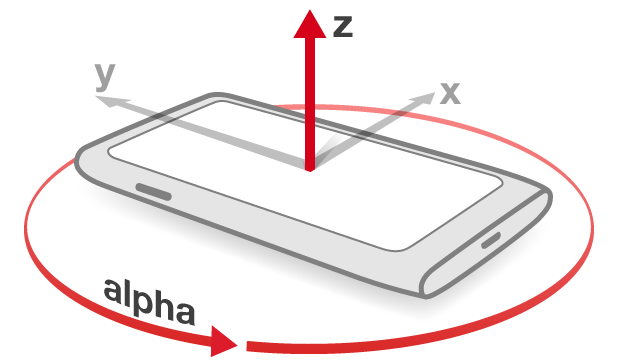
\includegraphics[scale=0.2]{img/device-alpha}
  \end{minipage}
  \hspace{1cm}
  \begin{minipage}[c]{.23\textwidth}
    \centering
    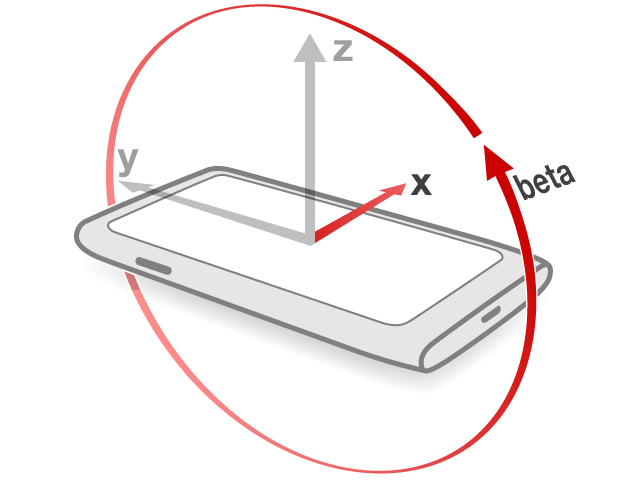
\includegraphics[scale=0.2]{img/device-beta}
  \end{minipage}
  \hspace{1cm}
  \begin{minipage}[c]{.23\textwidth}
    \centering
    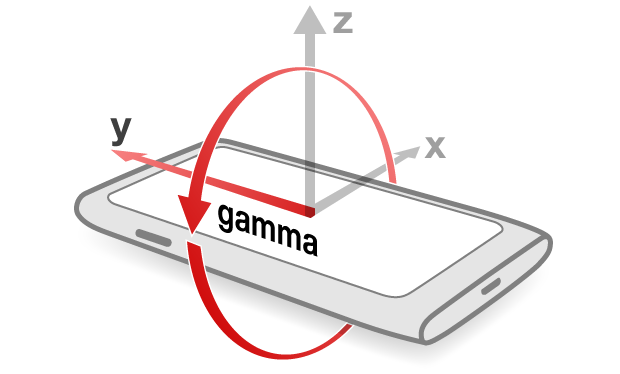
\includegraphics[scale=0.2]{img/device-gamma}
    \hspace{1cm}
  \end{minipage}
  \caption{The device rotation axes for the JavaScript \texttt{DeviceOrientation}}
  \label{fig:device-rot}
\end{figure}
Alpha is measured in the range of 0\degree to 360\degree around the z-axis, beta in in the range of -180\degree to 180\degree around x-axis and gamma in the range of -90\degree to 90\degree around y-axis.\\
\\
The JavaScript for measurements of the gyroscope:
\lstinputlisting{code/gyro-listener.js}
\cite[]{sensor:W3C}

\section{Measurement I - Motion}\label{sec:measurementI}
The first measurement had the purpose to test the accelerometer with and without the impact of gravity. This with the purpose to see if any of them where a better choice in terms of characteristics uniqueness in the devices.\\
The data were collected by developing a JavaScript web-page that used the listeners described in~\sectionref{subsec:accJS}. The test where completely diverse in sense of device platform and only required a browser installed and Internet connection. 
This only require that the measured device has Internet connection and a browser installed, no additional installations and completely cross-platform.\\
\\
The measurements required that the device where still on a flat surface, then started by pressed a button. It gathered 1000 samples of accelerometer data that where saved as a CSV-file for further analyzing. It also collected gyroscope data as well for possible future analyzing purposes. The screen-shots below shows the web-page while measuring and the right one when finished and ready to send. 
\begin{figure}[H]
  \hspace{-2cm}
  \centering
  \begin{minipage}[c]{.23\textwidth}
    \centering
    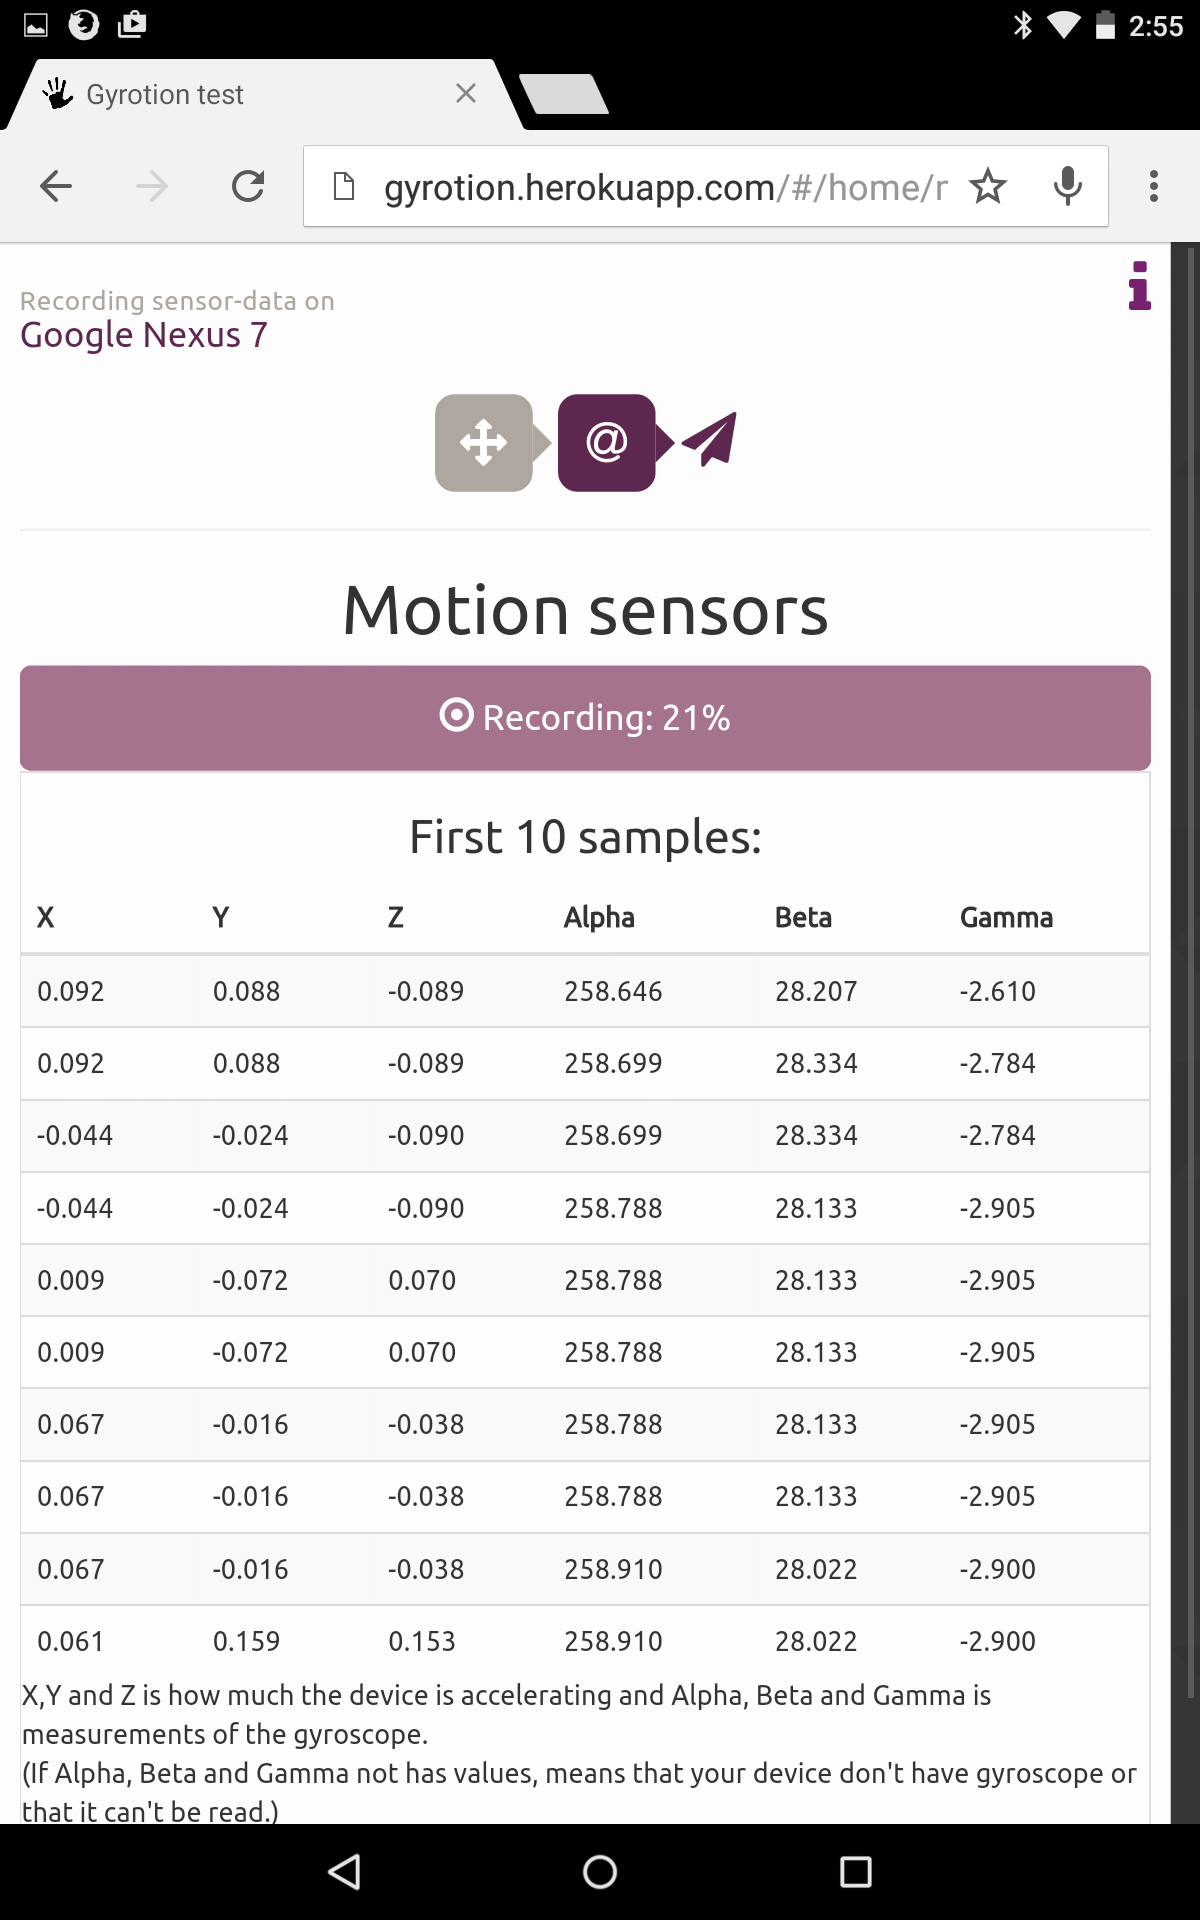
\includegraphics[scale=0.1]{img/Nexus-rec}
  \end{minipage}
  \hspace{2cm}
  \begin{minipage}[c]{.23\textwidth}
    \centering
    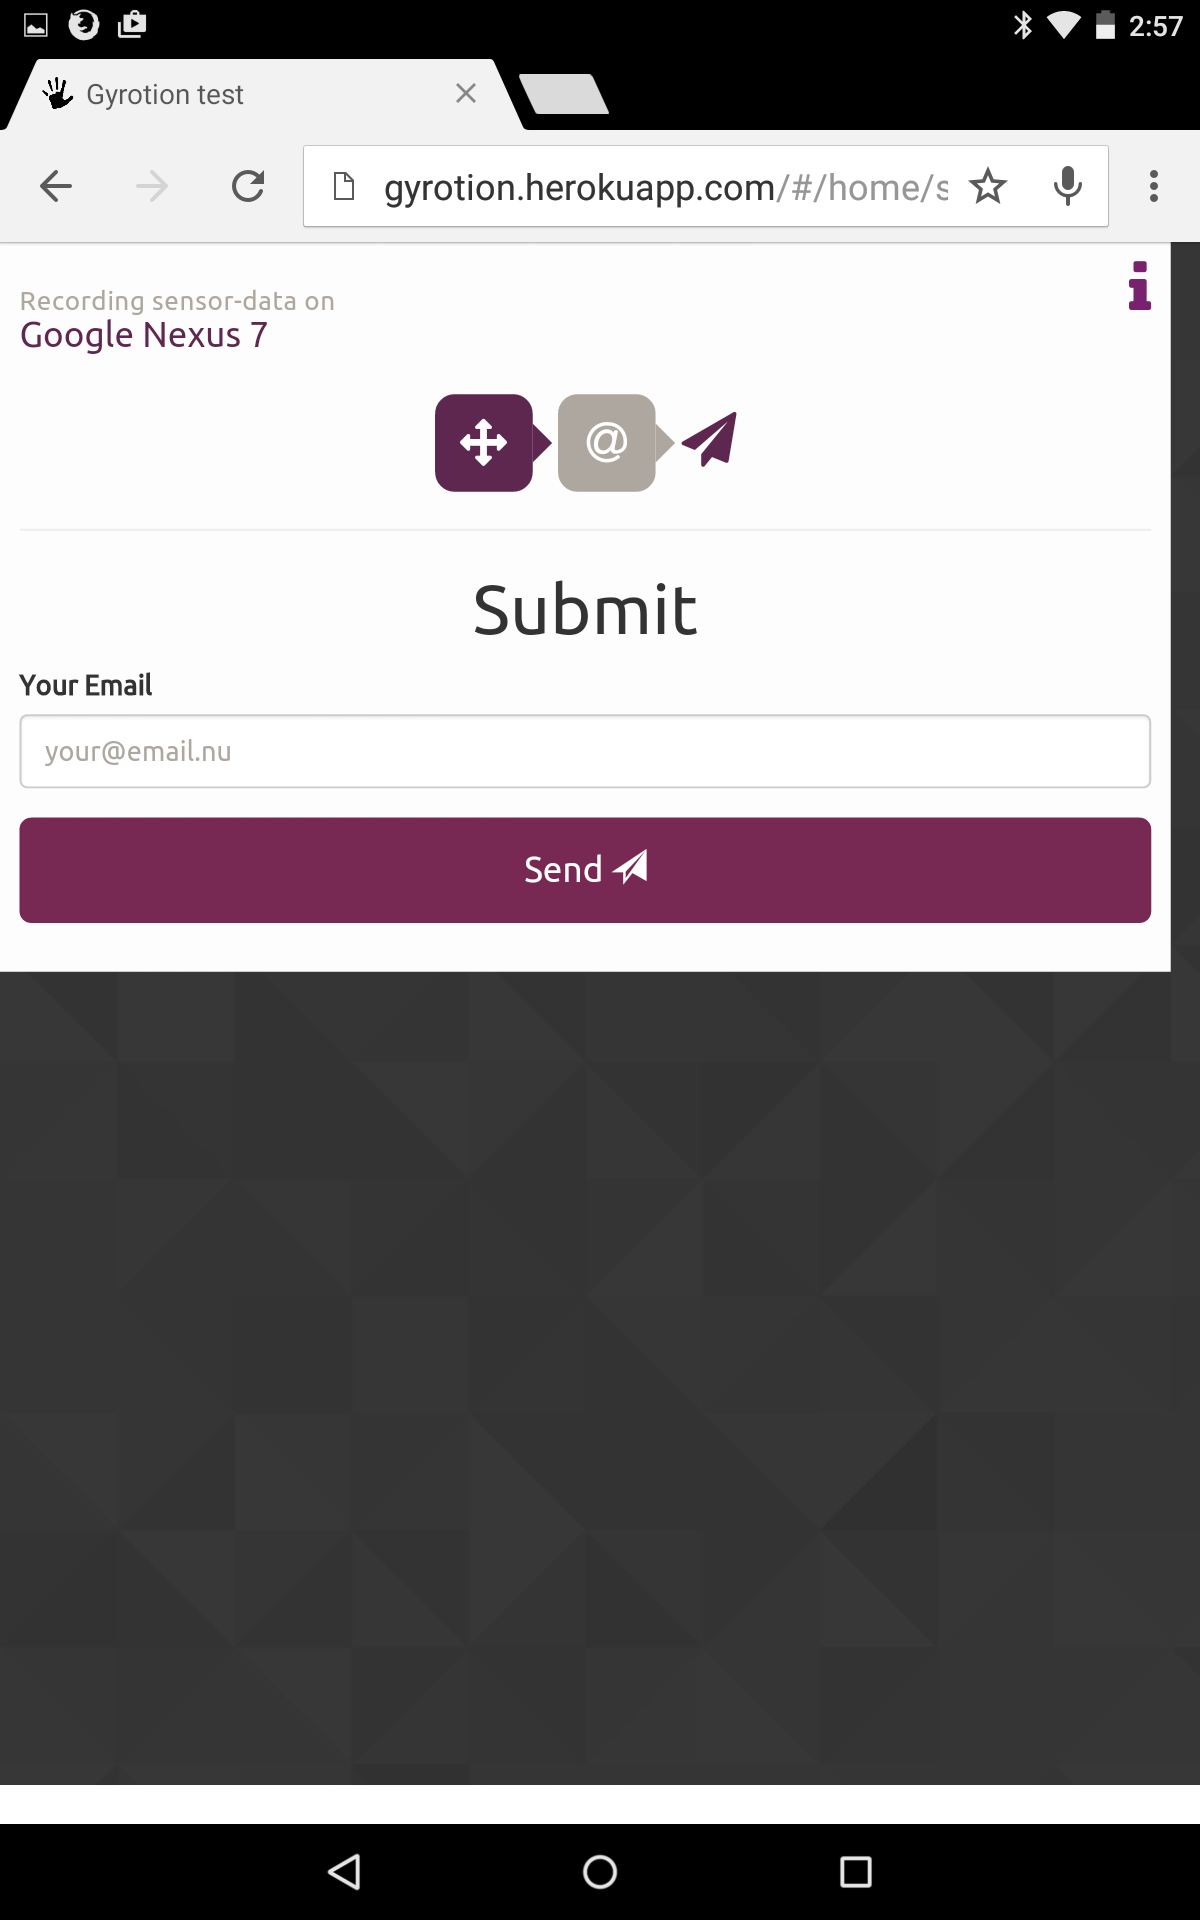
\includegraphics[scale=0.1]{img/Nexus-submit}
  \end{minipage}
  \caption{Screen-shots of web-page during accelerometer measurements in test I}
  \label{fig:gyrotion}
\end{figure}

\section{Measurement II - Motion}\label{sec:measurementII}
The second measurements where also performed from a web-page using JavaScript to collect gyroscope and accelerometer data and a file-upload to collect measurements from the camera of the device. As of the result in last test there where a few changes made to improve the accuracy of the measurements and to collect sensor samples from the gyroscope and camera:
\begin{enumerate}
  \item Adding time-stamp to every recording sample to know exactly recording frequency to enable further analyzing.
  \item Time based recording on 30 seconds instead of taking 1000 samples as in the first test (~\sectionref{sec:measurementI}).
  \item It's also sampling at a lower rate of at least 10 ms instead of as fast as it could before to reduce the effect of other processes that may are in use on the device.
  \item Accelerometer listener used is only \texttt{accelerationIncludingGravity}, due to results described in ~\sectionref{res:testI}.
  \item Added a listener for the gyroscope, ~\sectionref{subsec:gyroJS}.
  \item Collecting camera sensor by a five seconds black video, ~\sectionref{sec:measurement:camera}.
\end{enumerate}

\begin{figure}[H]
  \hspace{-2cm}
  \centering
  \begin{minipage}[c]{.23\textwidth}
    \centering
    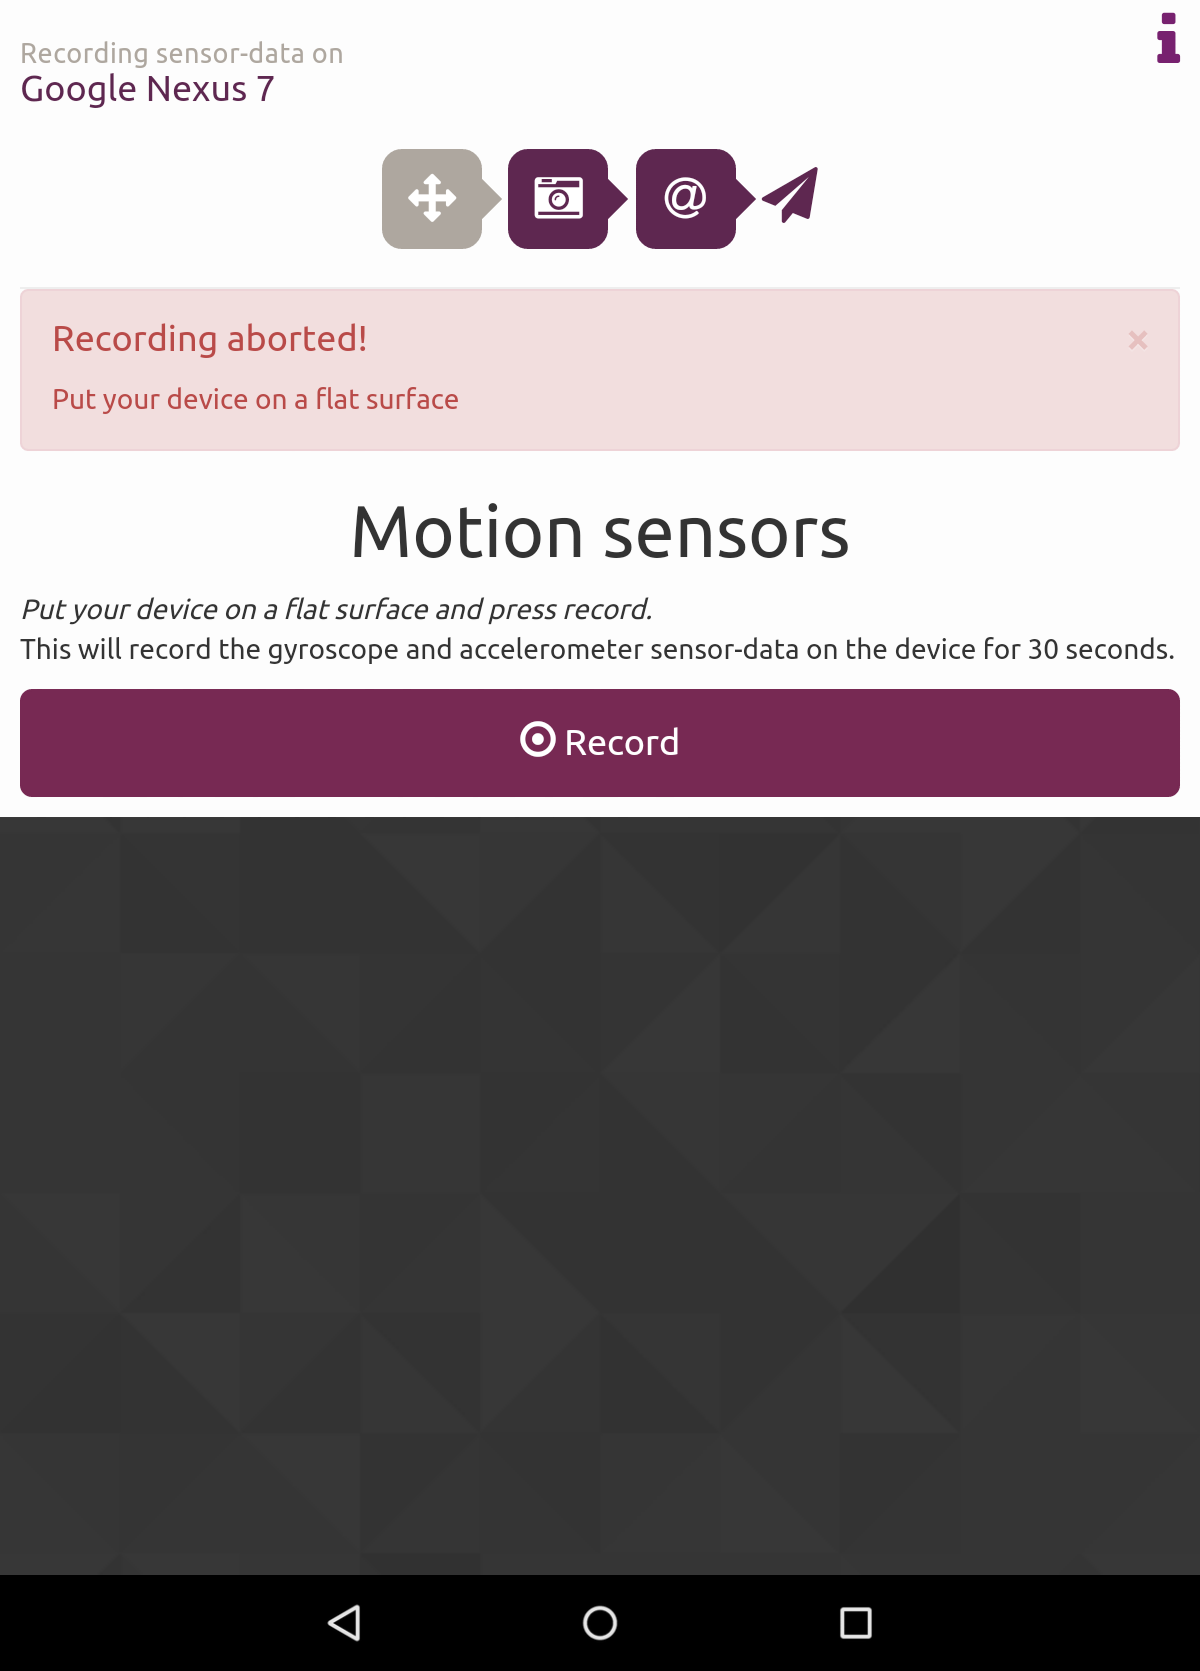
\includegraphics[scale=0.15]{img/sensorrec-nexus-2-notRec}
  \end{minipage}
  \hspace{2cm}
  \begin{minipage}[c]{.23\textwidth}
    \centering
    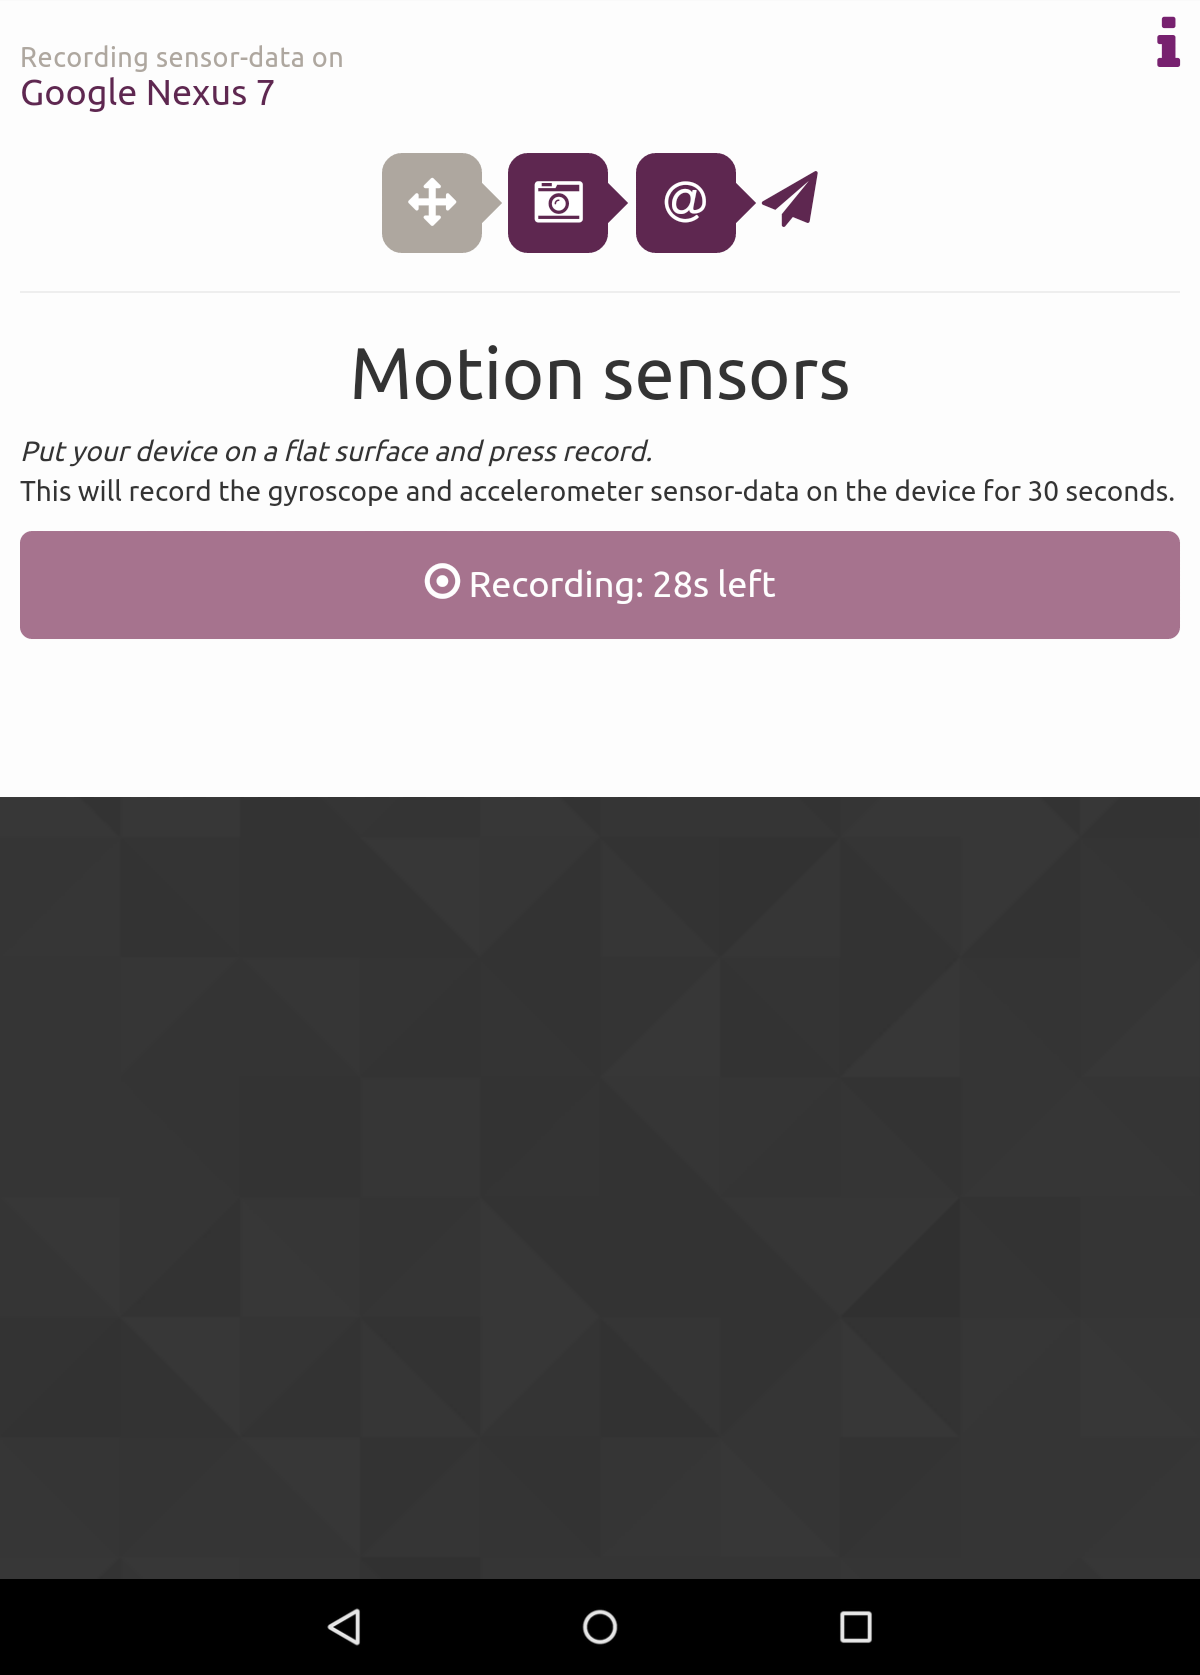
\includegraphics[scale=0.15]{img/sensorrec-nexus-1-rec}
  \end{minipage}
  \caption{Motion sensor measurements II on a Google Nexus 7}
  \label{fig:sensorrec}
\end{figure}

\section{Camera measurements}\label{sec:measurement:camera}
As most of the camera fingerprinting articles (REFERENSER!!) has mostly been in forensic purposes and not focusing on the measurability or integrity of the pictures. That is why some limitations has been made in these measurements. The black motive is used due to integrity, thus no information that could reveal the environment surrounding the camera is sent. Because of measurability (~\sectionref{auth:bio:character})) limited number of pictures that can be taken in a enrollment phase of a device fingerprinting authentication system.\\

To measure the camera two measurements where gathered in both cases where the device on a flat surface which makes the camera result black. Both of this measurements is analyzed by the PRNU-method used by~\cite{sensor:camera:DCIdent} described in~\sectionref{sec:ResCam}.
\begin{enumerate}
  \item \textbf{Black video:} The recommended number of pictures for camera fingerprinting is 50 ~\cite[]{sensor:camera:DCIdent}. But that is not a convenient gathering purposes, thus to ask someone to take 50 black photos and send will not make many answers. Thats why the first test asked for recording a 5 seconds video-recording with the camera towards a flat surface. This video is then shuttered into picture frames, 5 seconds generate 100-200 pictures depending on the recording rate of fps (frames per second).
  \item \textbf{10 black photos:} Simple as taking 10 photos, also with the camera pointing down on a flat surface. Since ~\cite{sensor:camera:DCIdent} where using pictures of diverse motive this aims to investigate if there may be enough with 10 pictures when the motive is the same.
\end{enumerate}

Screen-shots from the camera-page of the second measurements:
\begin{figure}[h!]
  \hspace{-2cm}
  \centering
  \begin{minipage}[c]{.23\textwidth}
    \centering
    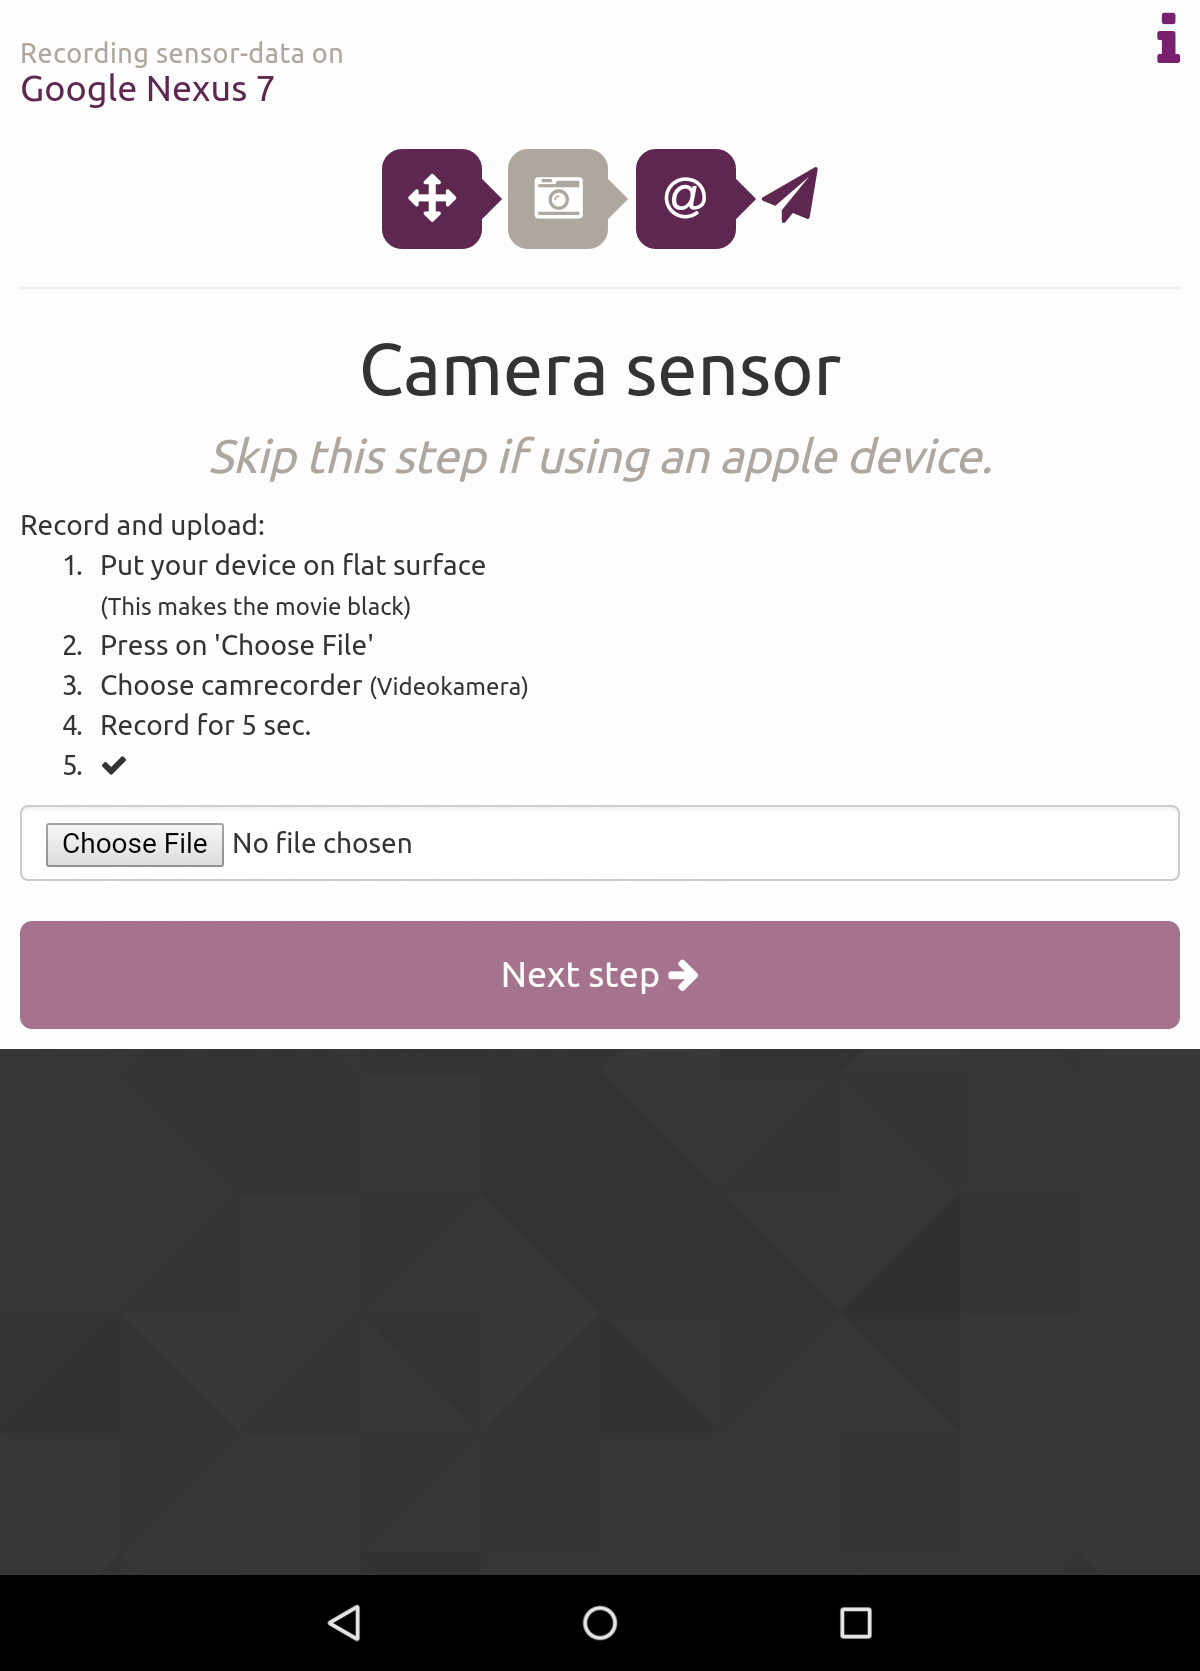
\includegraphics[scale=0.15]{img/sensorrec-nexus-3-cam}
  \end{minipage}
  \hspace{2cm}
  \begin{minipage}[c]{.23\textwidth}
    \centering
    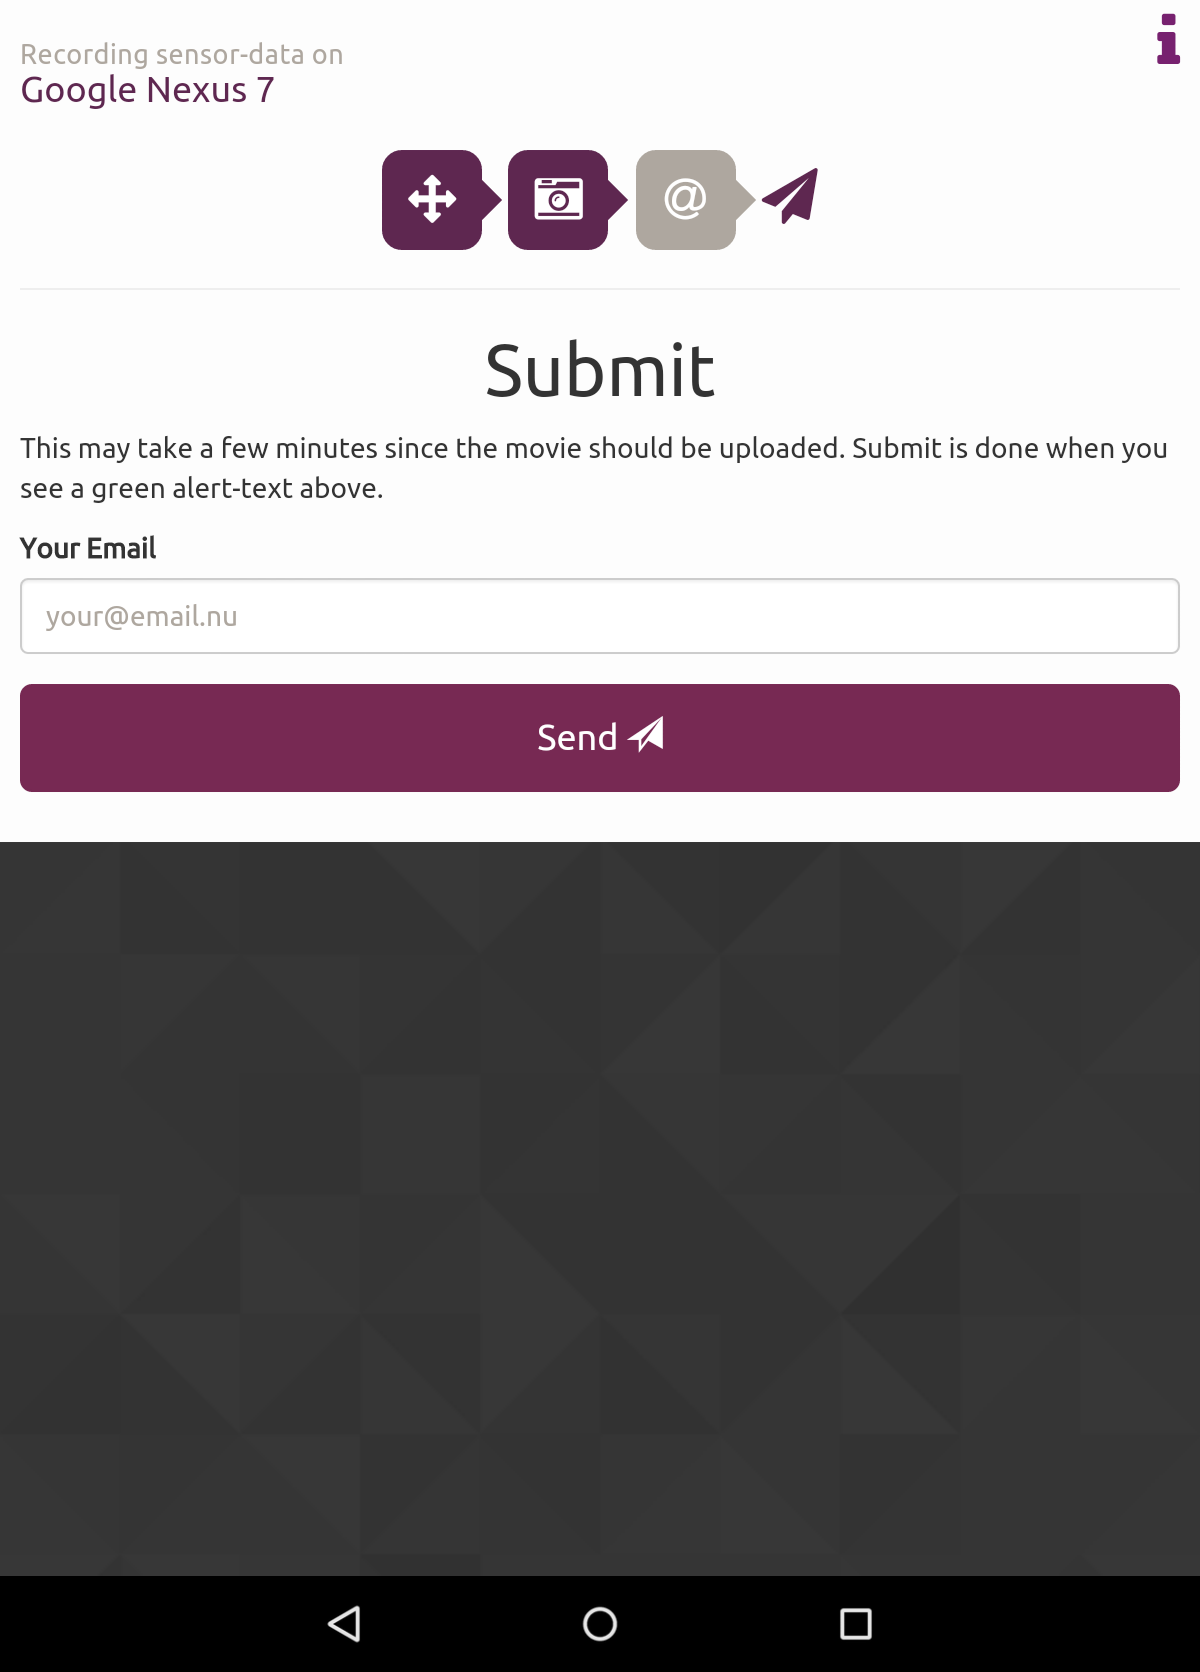
\includegraphics[scale=0.15]{img/sensorrec-nexus-4-send}
  \end{minipage}
  \caption{Sensor measurements on a Google Nexus 7}\label{fig:sensorrecCamera}
\end{figure}

For calculating the bias the MATLAB \texttt{medfilt2} is used, which is an 2-D median filtering that outputs the median value of each pixel by its 3-by-3 neighbors. 
\begin{figure}[H]
  \centering
  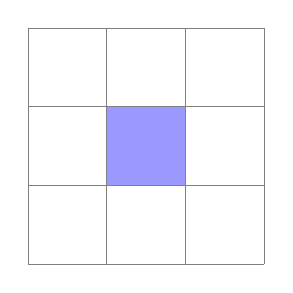
\begin{tikzpicture}[scale=1]
	\draw[step=1cm,gray,very thin] (0,0) grid (3,3);
	\fill[blue!40!white] (1,1) rectangle (2,2);
\end{tikzpicture}
  \caption{\label{fig:medfilt2} the MATLAB \texttt{medfilt2} outputs the median of each pixel by it's 3-by-3 neighbors}
\end{figure}
From the \texttt{medfilt2} is a picture gained without noise which is then subtracted from the original to get the noise. This technique works best if there are no features on the pictures such auto-fix, black and white etc. The more images used for the average value the better noise is, thus the amount random noise is less and the fixed noise is more. \cite{sensor:camera:DCIdent} recommend a minimum of 50 images. This is then seen as the reference pattern used for correlating the noise from another pictures. This correlation is calculated like:
$$
corr(\boldsymbol{n},\boldsymbol{r}) = 
\frac{(\boldsymbol{n} - \bar{\boldsymbol{n}})(\boldsymbol{r} - \bar{\boldsymbol{r}})}
{\|\boldsymbol{n} - \bar{\boldsymbol{n}}\| \|\boldsymbol{r} - \bar{\boldsymbol{r}}\|}
$$